% This is a LaTeX template kindly taken from Jernej Debevec.
% Provided by Miha Muskinja for the purpose of the seminar I in the 1st year
% of the 2nd cycle of the study of physics at the Faculty of Mathematics and Physics, University of Ljubljana.

% Set the document class and options
\documentclass[10pt, titlepage, a4paper]{article}
\usepackage[a4paper, inner=2.5cm, outer=2.5cm, top=2.25cm, bottom=2.25cm]{geometry}
\usepackage{graphicx}
\usepackage{hyperref}
\usepackage{wrapfig}
\usepackage{amsmath}
\usepackage{float}
\hypersetup{colorlinks=true}

% Load the natbib package for citation style
\usepackage{natbib}

% Some macros for commonly used symbols in physics/quantum mechanics
\newcommand{\bb}[1]{\bm#1}
\newcommand{\dd}{\mathrm{d}}
\newcommand{\pp}{\partial}
\newcommand{\dg}{\dagger}
\newcommand{\la}{\langle}
\newcommand{\ra}{\rangle}
\newcommand{\id}{\mathbb{1}}
\newcommand{\T}{\mathsf{T}}
\newcommand{\ua}{\uparrow\>}
\newcommand{\da}{\downarrow\>}
\newcommand{\fs}[1]{\slashed{#1}}  % Feynmann slash
\newcommand{\mc}[1]{\mathcal{#1}}
\newcommand\thickbar[1]{\accentset{\rule{.5em}{.03em}}{#1}}
\renewcommand{\bar}{\thickbar}

% Start the document
\begin{document}

% The title page
\begin{titlepage}
{\centering

\includegraphics[width=6cm]{logo_fmf.pdf}

\vspace{0.8cm}
{\small Department of Physics}

\vspace{5cm}
\vspace{0.5cm}
{\huge\textbf{Filtering and Spectral Analysis}} \\
\vspace{0.5cm}
{\large\textbf{10. Task for Model Analysis I, 2023/24}}

\vfill
\textbf{Author:} Marko Urbanč \\
\textbf{Professor:}  Prof. Dr. Simon Širca \\
\textbf{Advisor:}  doc. dr. Miha Mihovilovič\\

\vspace{1cm}
Ljubljana, August 2024 \\
}
\vspace{3cm}
\end{titlepage}

% Add table of conents
\hypersetup{pageanchor=true}
\pagenumbering{roman}
\setcounter{page}{2}
\tableofcontents
\vspace{1cm}

% Proceed with the main body
\pagenumbering{arabic}

% Sections based on typical Model Analysis structure
\section{Introduction}
Today we're taking a look at the filtering and spectral analysis of signals. Filtering is a process of removing unwanted parts of a signal,
while spectral analysis is a process of decomposing a signal into its frequency components. Both of these processes are crucial in signal processing and
would not be possible without the Fourier transform. The Fourier transform is a mathematical operation that transforms a function of time into a
function of frequency. It is used to represent the signal as a sum of sinusoidal functions from which we can extract important frequency information. The
equation for the Fourier transform and its inverse are given by:
%
\begin{gather}
    \hat{f}(\omega) = \frac{1}{\sqrt{2\pi}} \int_{-\infty}^{\infty} f(t) e^{-i\omega t} \dd t\>, \\
    f(t) = \frac{1}{\sqrt{2\pi}} \int_{-\infty}^{\infty} \hat{f}(\omega) e^{i\omega t} \dd \omega\>.~
\end{gather}
%
The Fourier transform has various properties that we've discussed in other tasks. What will turn out to be significant in this task is the fact that
the Fourier transform \textit{imagines/expects} that the input signal is periodic. This is important because the Fourier transform of a signal that is not
periodic will be subject to various effects of aliasing and leakage. These effects can be mitigated by windowing the signal before applying the Fourier
transform. Windowing is a process of multiplying the signal by a window function that is zero outside of a certain interval. This effectively
makes the signal periodic and reduces the effects of aliasing and leakage. Figure \ref{fig:windows} shows some common window functions that are used in
signal processing.

\begin{figure}[H]
    \centering
    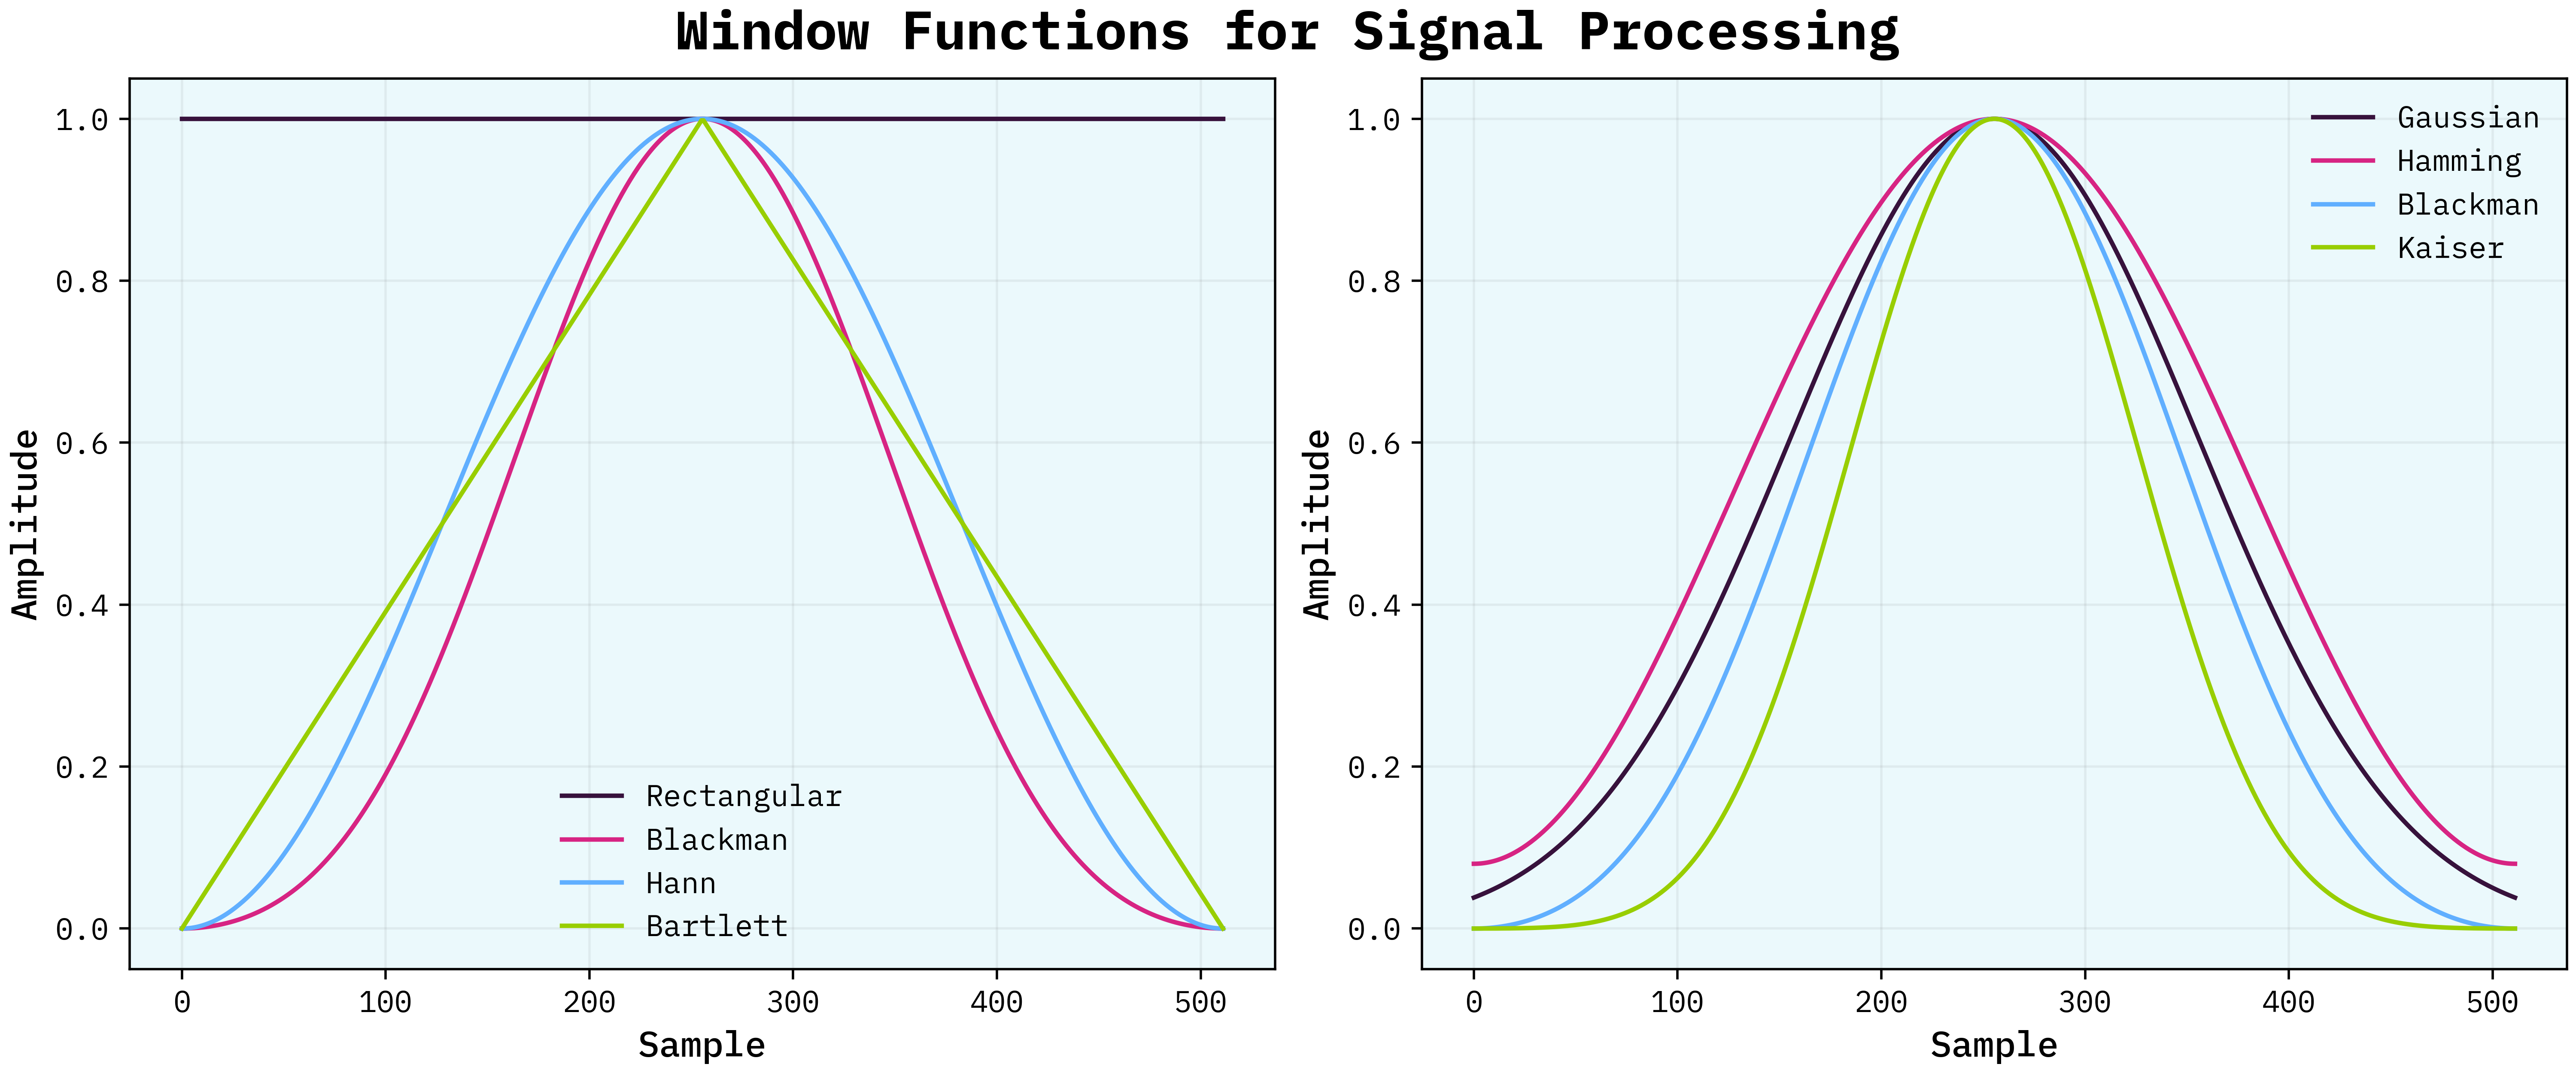
\includegraphics[width=0.98\textwidth]{../SpectralAnalysis/Images/window-functions.png}
    \caption{Common window functions used in signal processing.}
    \label{fig:windows}
\end{figure}

An important operation in signal processing is the convolution. Convolution is a mathematical operation that combines two signals to produce 
a third signal. It is used to model the effect of one signal on another signal. The convolution of two signals $f(t)$ and $g(t)$ is given by:
%
\begin{equation}
    (f * g)(t) = \int_{-\infty}^{\infty} f(\tau) g(t - \tau) \dd \tau\>.
\end{equation}
%
The convolution operation is commonly used in filtering. Filtering is a process of removing unwanted parts of a signal. Filters can be divided into roughly
two categories: low-pass filters and high-pass filters. Low-pass filters allow (or pass) low-frequency signals and block high-frequency signals, while high-pass
filters do the opposite. Filters can be implemented in the time domain or in the frequency domain. In the time domain, filters are implemented as convolution
operations, while in the frequency domain, filters are implemented as multiplication operations. For todays task we'll take a look at \textbf{Wiener's (Optimal) Filter}.
Wiener's filter is an optimal filter that minimizes the mean square error between the estimated random process (noise) and the desired process (signal). Imagine we
have a signal $u(t)$ which we measure using a sensor with the transfer function $r(t)$. The signal with the addition of noise $n(t)$ is then given by:
%
\begin{equation}
    c(t) = u(t) * r(t) + n(t) = s(t) + n(t)\>,
\end{equation}
%
where $*$ denotes the convolution operation. From the measured quantity $c(t)$ we want to reconstruct the signal $u(t)$, given the fact that we have some 
information on the noise $n(t)$ and the sensors response $r(t)$. Following analogously to the Least Squares method, Wiener proposed a filter in which we 
have to multiply the Fourier transform of the measured signal $\hat{c}(\omega)$  with:
%
\begin{equation}
    \Phi(\omega) = \frac{|\hat{s}(\omega)|^2}{|\hat{s}(\omega)|^2 + |\hat{n}(\omega)|^2}\>.
\end{equation}
%
We can also perform the so-called Wiener deconvolution using the Wiener filter and a convolution kernel (which is the transfer function of the sensor). So in 
the case of image restoration we can use the Wiener filter to remove the noise from the image if we know the transfer function of the sensor, which could for 
example be the point spread function of the camera with leads to blurring of the image. There are many other methods for image restoration, but 
Wiener's filter is a good starting point and we'll limit ourselves to this method in this task.

\section{Task}
\subsection{Spectra of Signals}
In the first subtask, the instructions want us to calculate the spectra of signals, that were provided in \texttt{val2.dat} and \texttt{val3.dat}. We should 
try out different windowing functions to see how they affect the spectra. We can also try and see what happens if we only select a part of the signal and
calculate the spectrum of that part. Figure \ref{fig:signals} shows the signals we've been given and their raw spectra.

\begin{figure}[h]
    \centering
    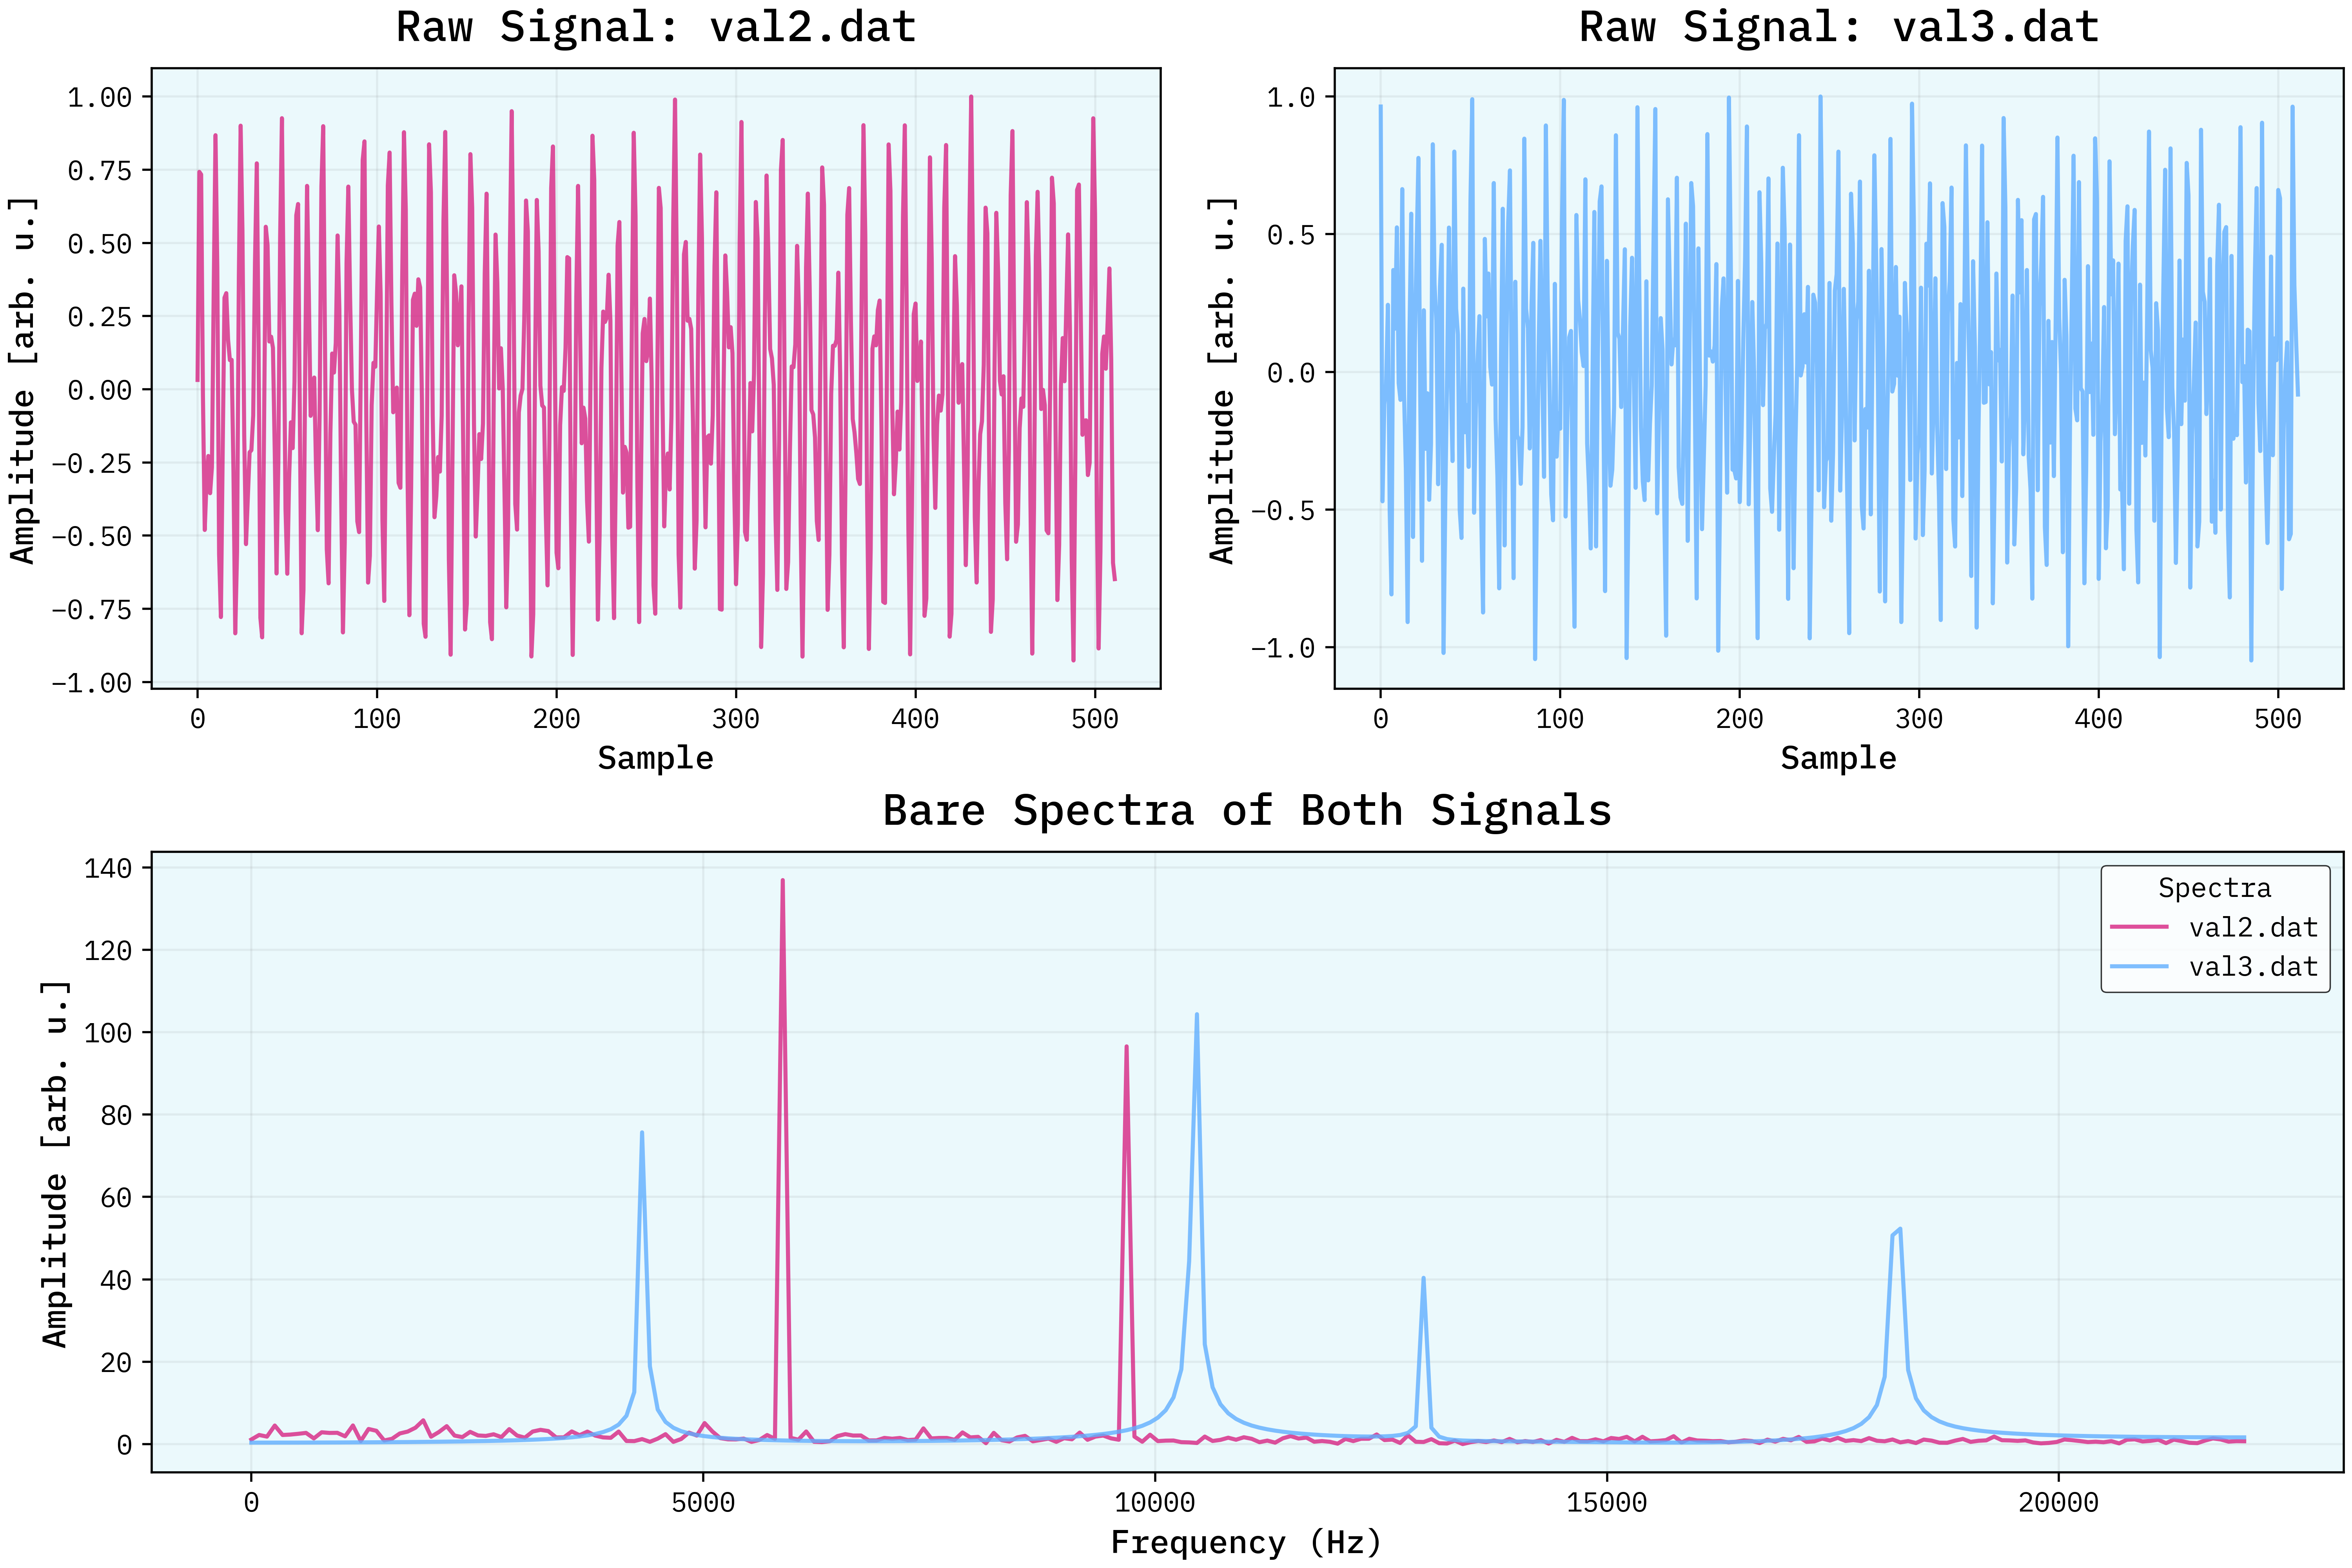
\includegraphics[width=0.98\textwidth]{../SpectralAnalysis/Images/raw-signals-spectra.png}
    \caption{Signals \texttt{val2.dat} and \texttt{val3.dat} and their raw spectra.}
    \label{fig:signals}
\end{figure}

\subsection{Wiener Filtering}
We have signals \texttt{signal\{0,1,2,3\}.dat} provided for the second task, each $512$ samples long.  Using Wiener's Filter we should try and 
remove the noise from the signals. \texttt{signal0.dat} represents the noiseless signal while the other signals have increasing levels of noise added to them.
The transfer function of the sensor is given by:
%
\begin{equation}
    r(t) = \frac{1}{2\tau} e^{-|t|/\tau}\>, \quad\quad\text{where}\quad\tau = 16\>.
\end{equation}
%
\subsection{Wieners Deconvolution}
For the last subtask we've received (cropped) images of Playboy model Lena Forsen (previously Soderberg). Her portrait called \texttt{Lenna} has become 
the standard test for various image processing algorithms and techniques. We've been given images of Lena that have been damaged by the addition of one of 
three convolution kernels and increasing levels of noise. The instructions want us to use Wiener's deconvolution to restore the images as best we can making sure 
to take care of artifacting due to a non-periodic signal by using either windowing or zero-padding. For the final challenge we we're also given images that 
have an additional periodic perturbation to them. We should try and remove the periodic perturbation from the images using some form of 
frequency domain filtering. Figure \ref{fig:lena} shows some of the images we've been given and their matching convolution kernels.

\begin{figure}[H]
    \centering
    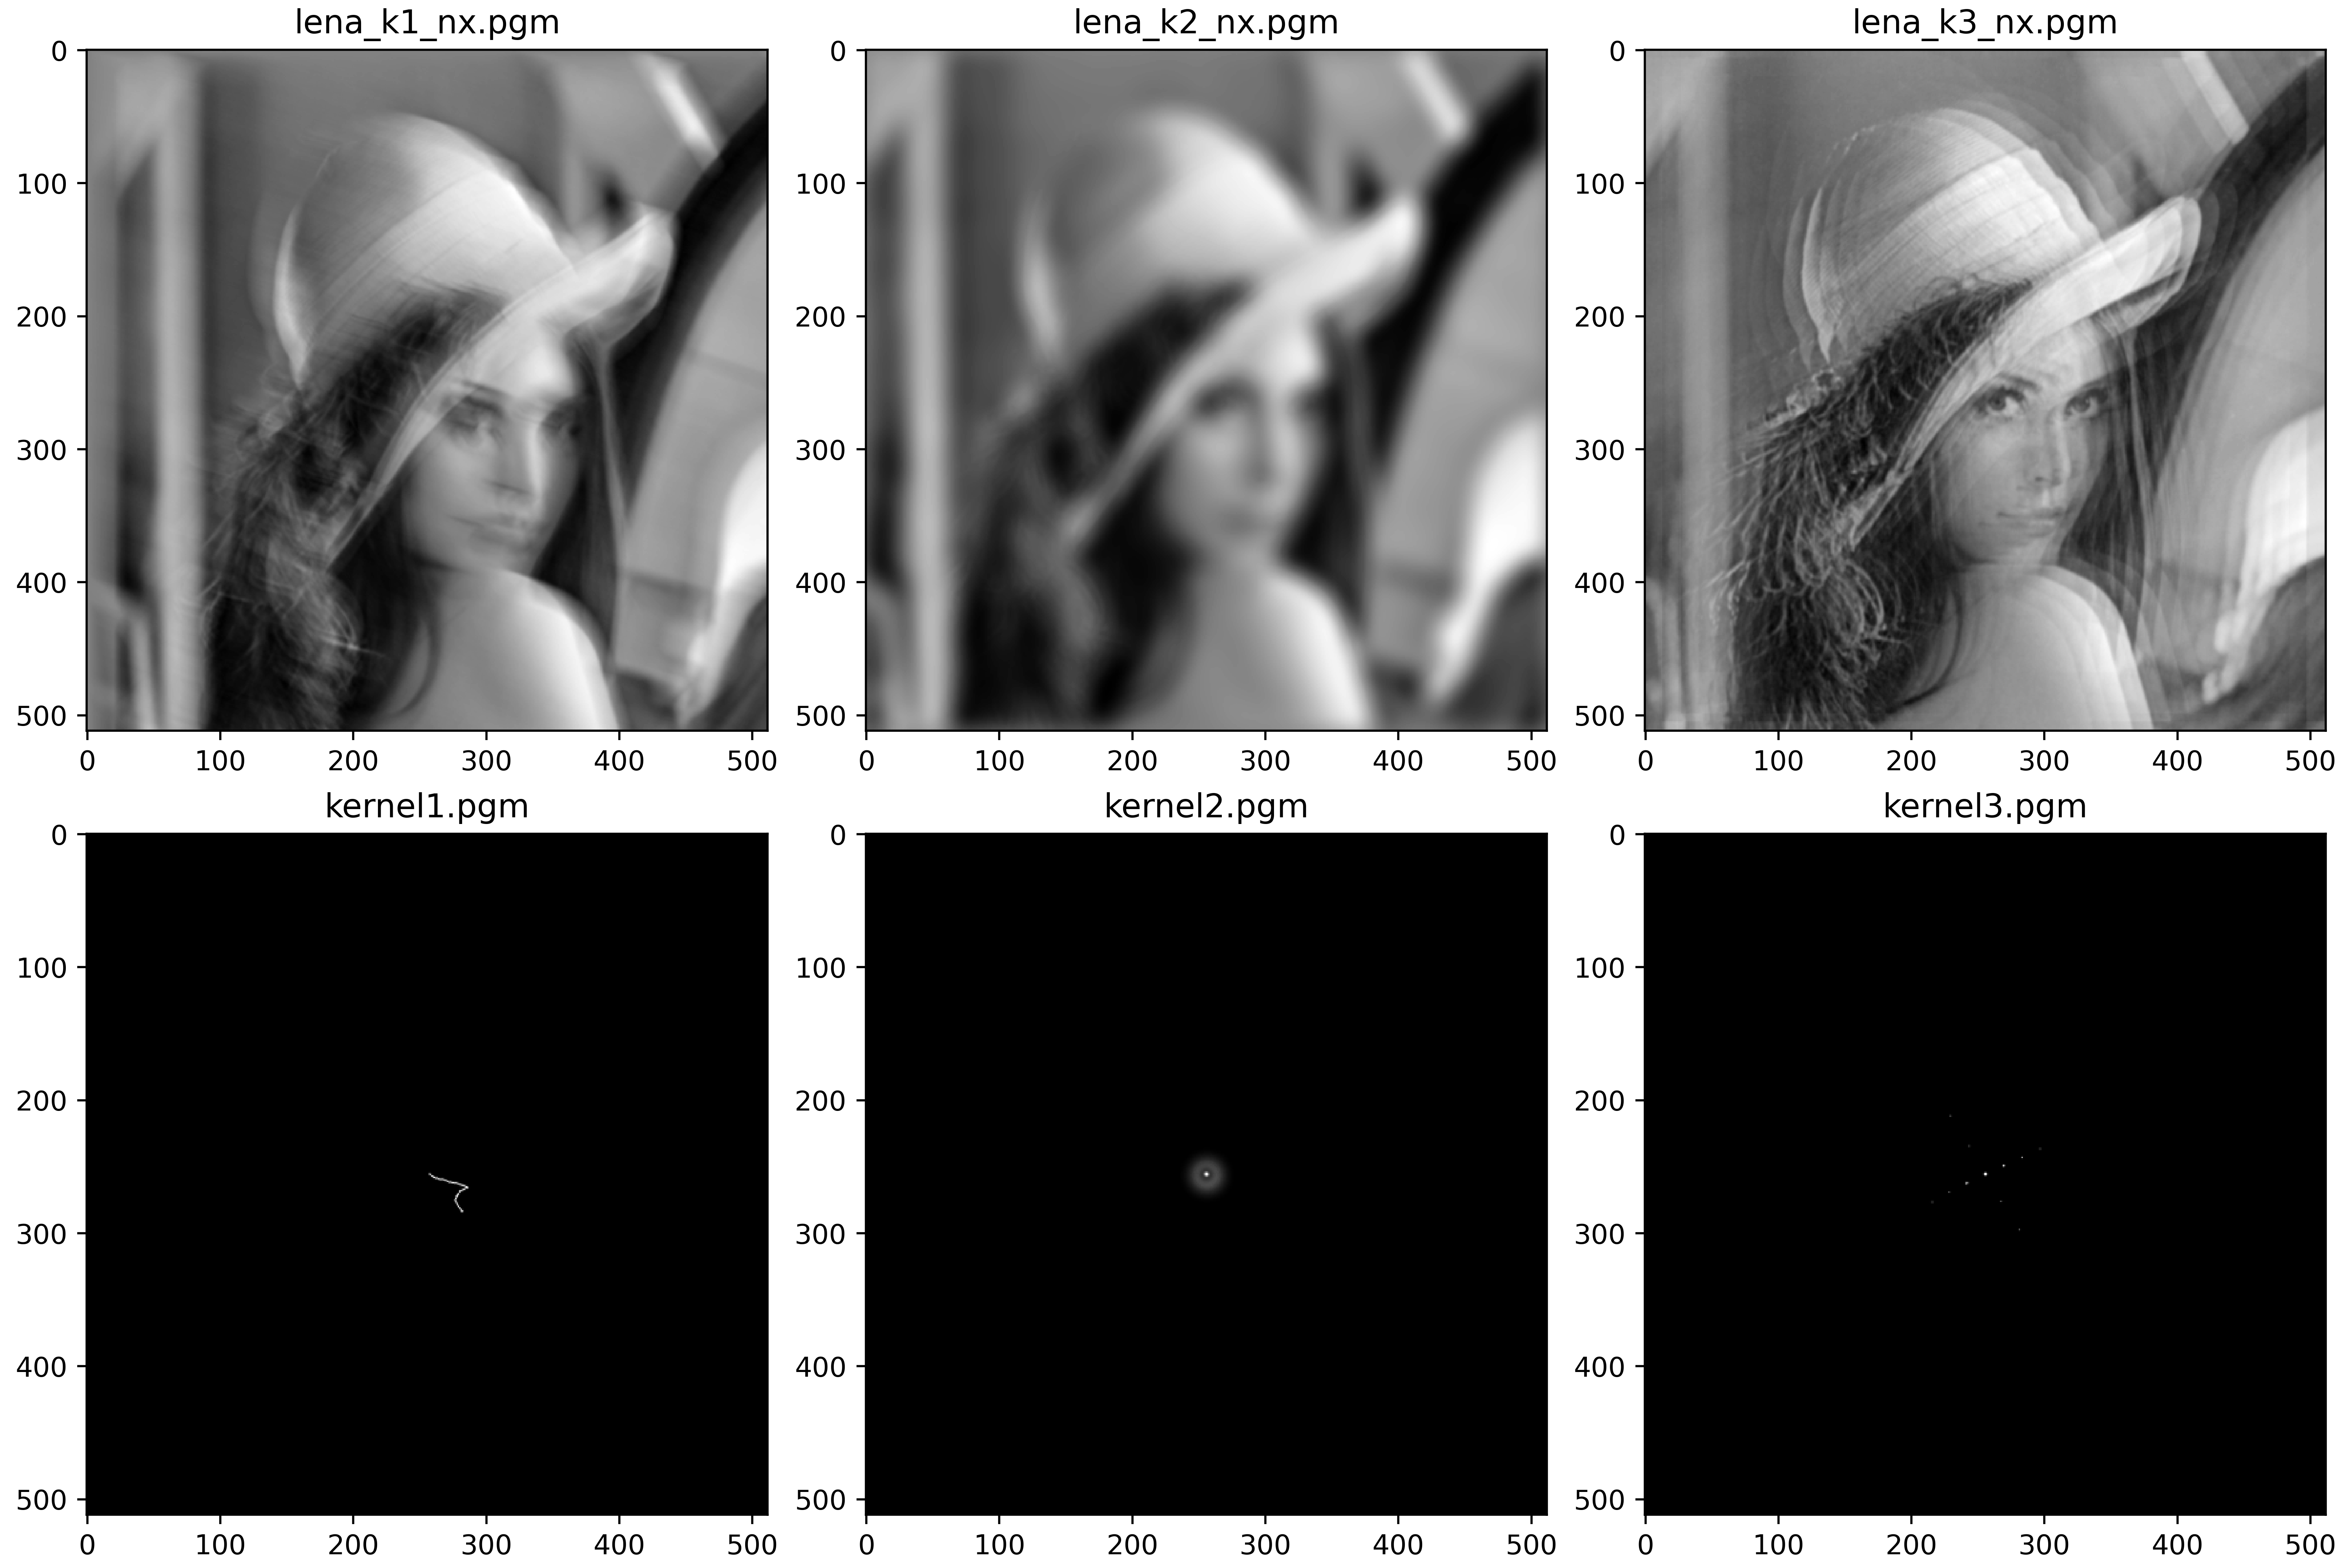
\includegraphics[width=0.98\textwidth]{../ImageDeconvolution/Images/lena_and_kernels.png}
    \caption{Images of Lena Forsen and their matching convolution kernels.}
    \label{fig:lena}
\end{figure}

\section{Solution Overview}
Another core mantra I want my stubborn brain to learn is to use already existing libraries and tools to solve problems. Sure I think it would be much more 
educational to write all the presented methods from scratch but that is unfortunately time consuming and thus not very practical. As this task doesn't really 
include bulk data gathering I also didn't make use of any multiprocessing, threading or distributed computing via say a package like \texttt{ray}. Besides the 
Python data science gold standard \texttt{numpy} and \texttt{scipy} I also used \texttt{scikit-image} for its plethora of already implemented image processing 
algorithms. Especially the submodule \texttt{skimage.restoration} was very useful as it already contains both Wiener's filter and Wiener's deconvolution. The rest 
of the task was mostly about reading in the data, applying and adjusting the filters etc. and plotting the results using \texttt{matplotlib}. As I didn't do any parameter 
scans I didn't really se the use of taking a class-based approach.
\section{Results}
\subsection{Spectra of Signals}
The spectra of the signals \texttt{val2.dat} and \texttt{val3.dat} are shown in Figure \ref{fig:signals}. We can see very clearly the prominent peaks in the spectra.
It is also evident that peaks in \texttt{val3.dat} are much wider than in \texttt{val2.dat}. I assume they are subject to leakage effects due to the 
signal end-points not matching this making the signal non-periodic. 

\section{Conclusion and Comments}

% Add references
% \newpage
% \bibliographystyle{unsrt}
% \bibliography{mod110}

% End document
\end{document}
